\subsection*{Exercício 3}
\addcontentsline{toc}{subsection}{Exercício 3}

Este exercício utiliza o dataset MNIST para comparar diferentes algoritmos de classificação de dígitos manuscritos.

\subsubsection*{Configuração inicial e carregamento dos dados}

\begin{lstlisting}[language=Python]
from sklearn.datasets import fetch_openml
from sklearn.neighbors import KNeighborsClassifier
from sklearn.naive_bayes import BernoulliNB
from sklearn.discriminant_analysis import LinearDiscriminantAnalysis
from sklearn.discriminant_analysis import QuadraticDiscriminantAnalysis
from sklearn.linear_model import LogisticRegression
from sklearn.ensemble import RandomForestClassifier
from sklearn.neural_network import MLPClassifier
from sklearn.metrics import confusion_matrix
from sklearn import svm
from sklearn.model_selection import train_test_split
import numpy as np
import matplotlib.pyplot as plt

def plot_digits(
    images,
    n_rows=2,
    n_cols=5,
    fig_shape=(20, 8),
    indexes=[0, 1, 2, 3, 4, 5, 6, 7, 8, 9],
    img_shape=(28, 28),
    labels=[0, 1, 2, 3, 4, 5, 6, 7, 8, 9],
):
    fig, axs = plt.subplots(n_rows, n_cols, figsize=fig_shape)
    ind = np.array(indexes).reshape(n_rows, n_cols)
    if labels:
        plt_labels = np.array(labels).reshape(n_rows, n_cols)
    for i in range(0, n_rows):
        for j in range(0, n_cols):
            if labels:
                axs[i, j].set_title(plt_labels[i, j], fontsize=20)
            axs[i, j].imshow(
                (images[ind[i, j]].reshape(img_shape)), cmap="plasma"
            )
            axs[i, j].axis("off")

mnist = fetch_openml("mnist_784")  # Baixar os dados
X, y = mnist.data.to_numpy(), mnist.target.to_numpy()
X = X / 255  # Colocar as features em [0, 1]
# Divisão em treino e teste
X_train, X_test, y_train, y_test = train_test_split(
    X, y, test_size=0.2, random_state=42
)
# Plot dos dígitos
plot_digits(
    X, n_rows=2, n_cols=5, indexes=[21, 24, 16, 27, 26, 35, 13, 15, 17, 19]
)
\end{lstlisting}

\begin{figure}[H]
    \centering
    \includegraphics[width=0.8\textwidth]{../figures/3/mnist_samples.png}
    \caption{Exemplos de dígitos do dataset MNIST}
    \label{fig:mnist_samples}
\end{figure}

\subsubsection*{(a) Comparação de modelos: acurácia e tempo de execução}

\begin{lstlisting}[language=Python]
from sklearn.metrics import accuracy_score
import time

nb = BernoulliNB(force_alpha=True)  # Naive Bayes com features bernoulli
lda = LinearDiscriminantAnalysis()  # LDA
qda = QuadraticDiscriminantAnalysis(reg_param=0.01)  # QDA
lr = LogisticRegression(random_state=42)  # Regressão Logística
knn = KNeighborsClassifier(n_neighbors=6)  # kNN com k = 6
svc = svm.SVC(gamma="scale", class_weight="balanced", C=100)  # SVM
rf = RandomForestClassifier(
    max_depth=30, random_state=0, n_estimators=100
)  # Random forest
nn = MLPClassifier(
    random_state=42, hidden_layer_sizes=[100], max_iter=300
)  # Rede neural

models = [nb, lda, qda, lr, knn, svc, rf, nn]

yhats = []
accuracy = []
time_train = []
time_test = []
i = 0
for model in models:
    start_time = time.time()
    model.fit(X_train, y_train)
    end_time = time.time()
    time_train.append(end_time - start_time)

    start_time = time.time()
    yhat = model.predict(X_test)
    end_time = time.time()
    time_test.append(end_time - start_time)

    yhats.append(yhat)
    accuracy.append(accuracy_score(y_true=y_test, y_pred=yhat))
    i += 1
\end{lstlisting}

\textbf{Resultados de acurácia e tempo de execução:}

\begin{table}[H]
    \centering
    \begin{tabular}{|l|c|c|c|}
        \hline
        \textbf{Modelo}     & \textbf{Acurácia} & \textbf{Tempo Treino (s)} & \textbf{Tempo Teste (s)} \\
        \hline
        Naive Bayes         & [ACURACIA\_NB]    & [TEMPO\_TREINO\_NB]       & [TEMPO\_TESTE\_NB]       \\
        LDA                 & [ACURACIA\_LDA]   & [TEMPO\_TREINO\_LDA]      & [TEMPO\_TESTE\_LDA]      \\
        QDA                 & [ACURACIA\_QDA]   & [TEMPO\_TREINO\_QDA]      & [TEMPO\_TESTE\_QDA]      \\
        Regressão Logística & [ACURACIA\_LR]    & [TEMPO\_TREINO\_LR]       & [TEMPO\_TESTE\_LR]       \\
        kNN                 & [ACURACIA\_KNN]   & [TEMPO\_TREINO\_KNN]      & [TEMPO\_TESTE\_KNN]      \\
        SVM                 & [ACURACIA\_SVM]   & [TEMPO\_TREINO\_SVM]      & [TEMPO\_TESTE\_SVM]      \\
        Random Forest       & [ACURACIA\_RF]    & [TEMPO\_TREINO\_RF]       & [TEMPO\_TESTE\_RF]       \\
        Rede Neural         & [ACURACIA\_NN]    & [TEMPO\_TREINO\_NN]       & [TEMPO\_TESTE\_NN]       \\
        \hline
    \end{tabular}
    \caption{Comparação de acurácia e tempos de execução dos modelos}
    \label{tab:model_comparison}
\end{table}

\textbf{Observações:}
\begin{itemize}
    \item Para a convergência do modelo de QDA, foi necessário adicionar um parâmetro de regularização \texttt{reg\_param = 0.01}.
    \item Os dados não foram normalizados, dada a escala semelhante das features.
\end{itemize}

\subsubsection*{(b) Análise da interpretabilidade dos modelos}

Para cada um dos gráficos gerados pelos códigos abaixo, explicamos o que está sendo mostrado, como isso se relaciona com as previsões do modelo em questão e se é possível interpretar com facilidade o que está acontecendo.

\textbf{(i) Parâmetros do Naive Bayes}

\begin{lstlisting}[language=Python]
nb_params = {}
for i in range(10):
    nb_params[i] = np.exp(nb.feature_log_prob_[i])

plot_digits(nb_params)
\end{lstlisting}

\begin{figure}[H]
    \centering
    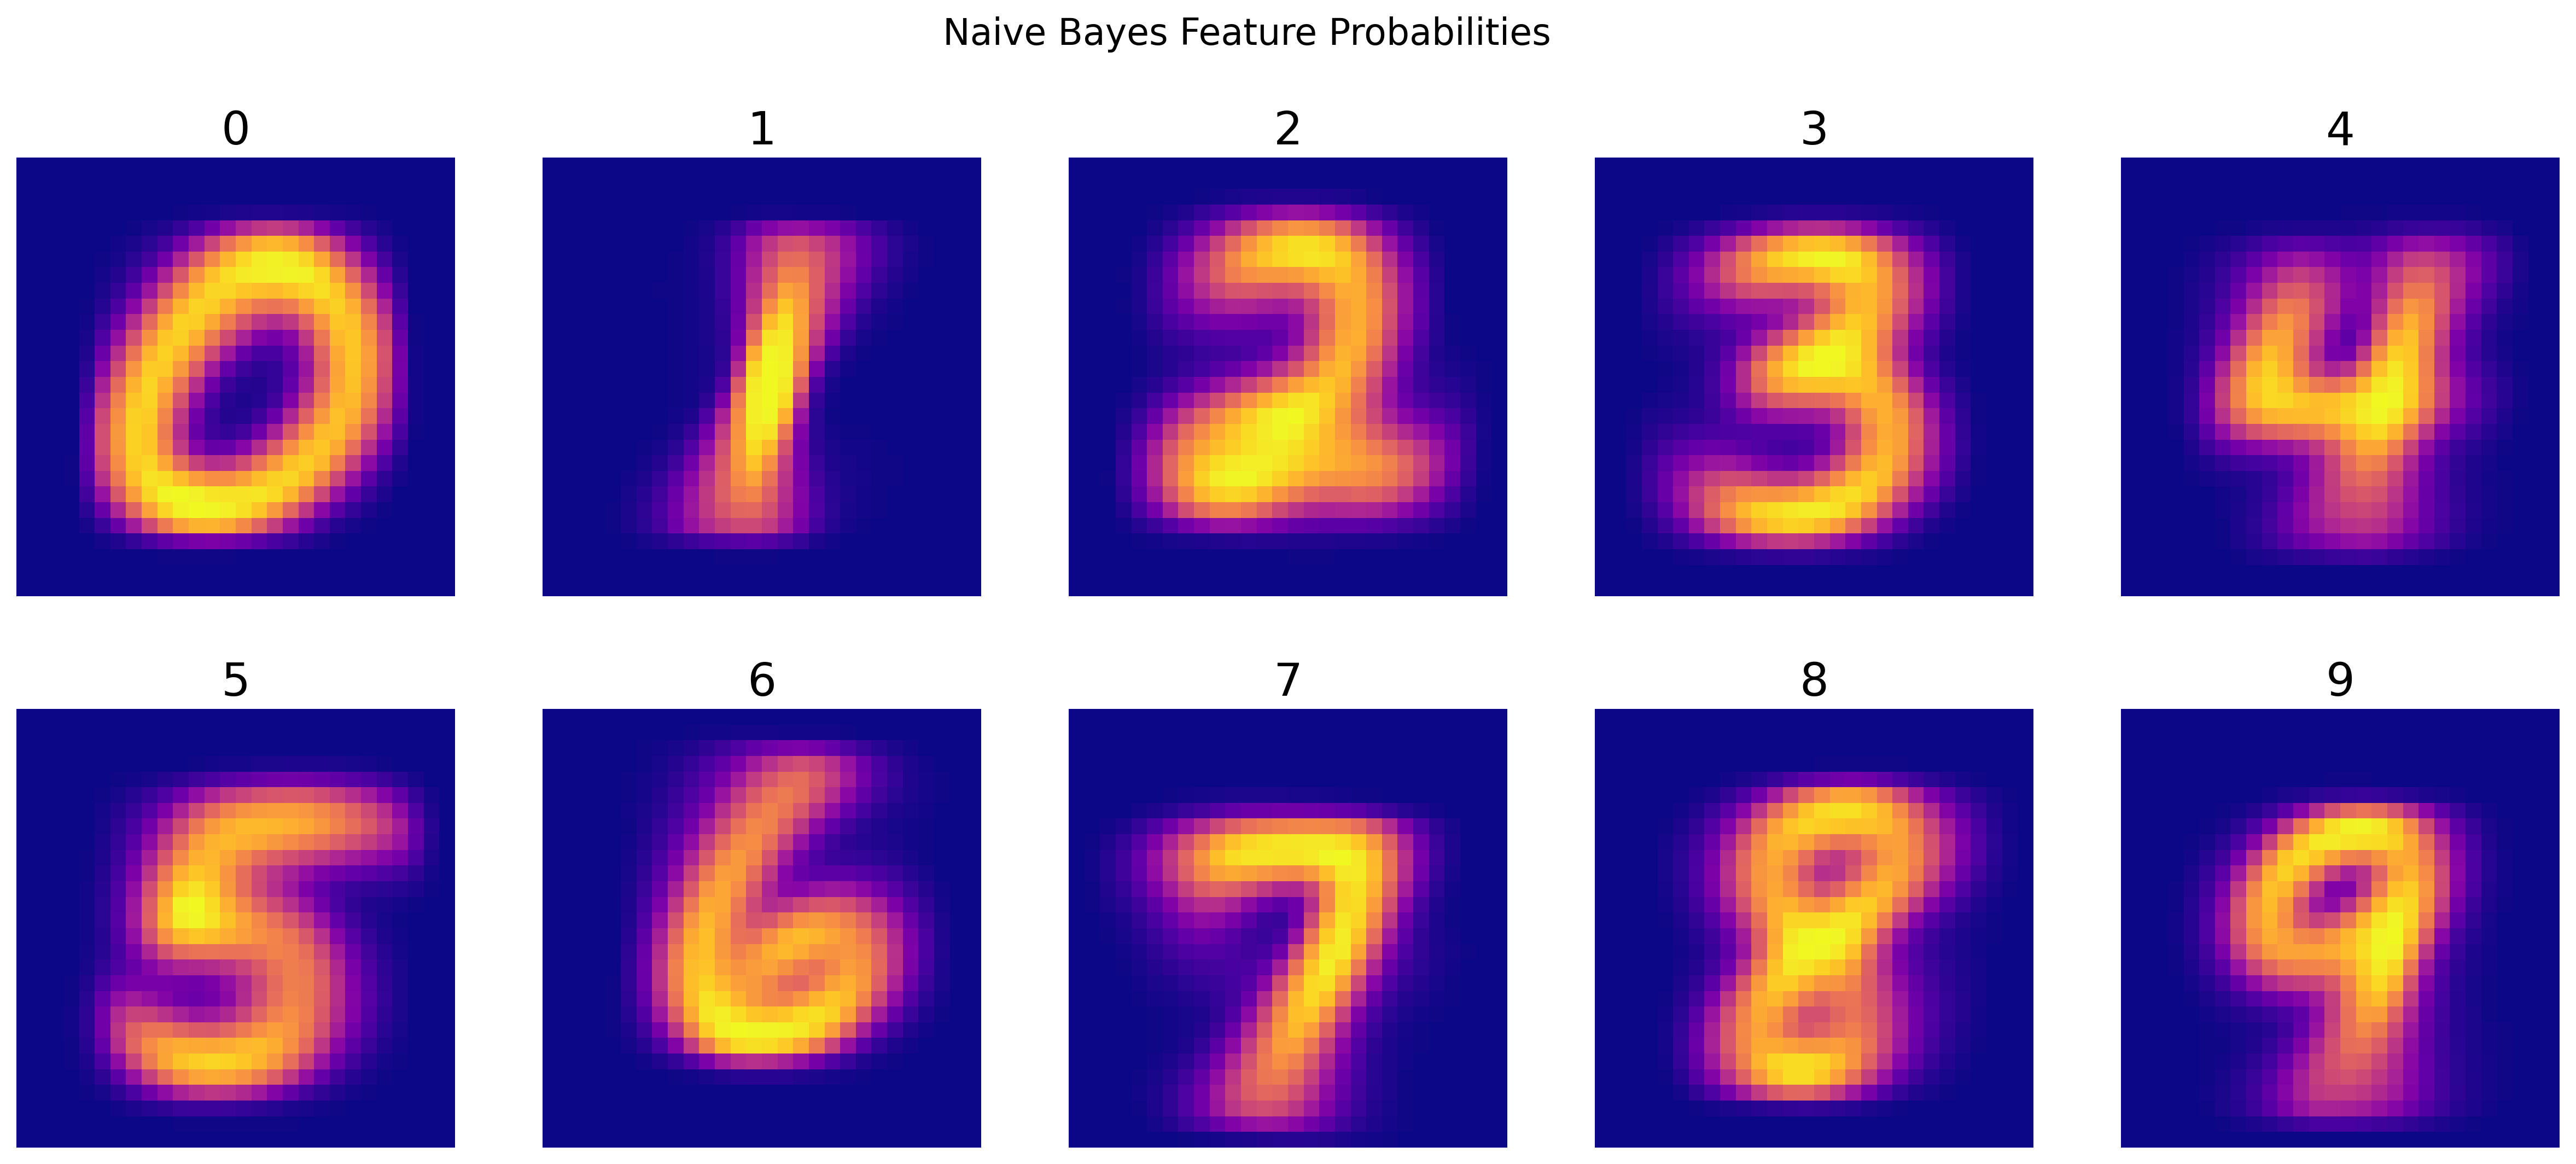
\includegraphics[width=0.8\textwidth]{../figures/3/naive_bayes_params.png}
    \caption{Probabilidades dos pixels para cada classe no modelo Naive Bayes}
    \label{fig:nb_params}
\end{figure}

Cada imagem representa a probabilidade dos pixels da imagem pertencerem à respectiva classe, sendo que valores altos indicam pixels recorrentes para a classe. O produto entre este vetor e a entrada indicará a probabilidade da entrada ser pertencente à classe e será utilizada para classificação. A interpretação da imagem é simples e permite a reconstituição do dígito ao qual a classe referencia.

\textbf{(ii) Parâmetros do LDA}

\begin{lstlisting}[language=Python]
lda_params = {}
for i in range(10):
    lda_params[i] = lda.means_[i]

plot_digits(lda_params)
\end{lstlisting}

\begin{figure}[H]
    \centering
    \includegraphics[width=0.8\textwidth]{../figures/3/lda_means.png}
    \caption{Médias das classes no modelo LDA}
    \label{fig:lda_means}
\end{figure}

Cada uma das imagens é a média da respectiva classe no espaço de entrada. Essa imagem seria equivalente a uma amostra média, ponto central em relação às demais amostras da classe. As previsões do modelo baseiam-se em uma métrica de similaridade da entrada em relação a cada uma dessas médias. É possível interpretar com facilidade a classe relacionada a cada imagem.

\textbf{(iii) Parâmetros da Regressão Logística}

\begin{lstlisting}[language=Python]
log_reg_params = {}
for i in range(10):
    log_reg_params[i] = lr.coef_[i]

plot_digits(log_reg_params)
\end{lstlisting}

\begin{figure}[H]
    \centering
    \includegraphics[width=0.8\textwidth]{../figures/3/logistic_regression_coefs.png}
    \caption{Coeficientes do modelo de Regressão Logística}
    \label{fig:lr_coefs}
\end{figure}

A imagem representa o coeficiente da rede. Ao multiplicarmos pela entrada, teremos o logaritmo da probabilidade da amostra pertencer à classe sobre a probabilidade dela pertencer à classe de referência. A imagem mostrada é a resposta do modelo a uma matriz de 1's. Isso pode ser interpretado como a contribuição de cada pixel para a probabilidade final. Ainda mantemos uma interpretação válida de cada classe por meio da imagem, apesar de menos clara caso comparemos com as imagens dos modelos anteriores.

\textbf{(iv) Importância das features no Random Forest}

\begin{lstlisting}[language=Python]
rf_params = rf.feature_importances_.reshape(28, 28)

plt.axis("off")
plt.imshow(rf_params, cmap="plasma")
\end{lstlisting}

\begin{figure}[H]
    \centering
    \includegraphics[width=0.6\textwidth]{../figures/3/random_forest_importance.png}
    \caption{Importância das features no modelo Random Forest}
    \label{fig:rf_importance}
\end{figure}

A imagem representa a importância de cada pixel para o modelo, baseada na média do decaimento de uma métrica de impureza, no caso, o coeficiente de Gini. Valores altos indicam que aquela feature foi capaz de auxiliar na distinção entre as classes. Nesse caso, perde-se a interpretação individual das classes, entretanto ainda está clara qual a região mais importante para a classificação.

\textbf{(v) Parâmetros da Rede Neural}

\textbf{(v.a) Pesos da camada de entrada para a camada oculta}

\begin{lstlisting}[language=Python]
nn_params_1 = {}
for i in range(100):
    nn_params_1[i] = nn.coefs_[0][:, i]

indexes = list(range(100))

plot_digits(
    nn_params_1,
    n_rows=10,
    n_cols=10,
    fig_shape=(100, 100),
    indexes=indexes,
    img_shape=(28, 28),
    labels=None,
)
\end{lstlisting}

\begin{figure}[H]
    \centering
    \includegraphics[width=0.9\textwidth]{../figures/3/neural_network_layer1_weights.png}
    \caption{Pesos da camada de entrada para a camada oculta na Rede Neural}
    \label{fig:nn_layer1}
\end{figure}

Cada imagem representa os pesos que ligam a entrada a cada um dos neurônios da camada oculta. Eles são a transformação linear da entrada antes da primeira função de ativação e podem ser interpretados como parte de uma engenharia de features. A interpretabilidade já se perdeu completamente, tanto pela alta quantidade de neurônios quanto pela dificuldade de encontrar valor semântico em cada transformação.

\textbf{(v.b) Pesos da camada oculta para a camada de saída}

\begin{lstlisting}[language=Python]
nn_params_2 = {}
for i in range(10):
    nn_params_2[i] = nn.coefs_[1][:, i]

plot_digits(
    nn_params_2, n_rows=2, n_cols=5, fig_shape=(20, 8), img_shape=(10, 10)
)
\end{lstlisting}

\begin{figure}[H]
    \centering
    \includegraphics[width=0.8\textwidth]{../figures/3/neural_network_layer2_weights.png}
    \caption{Pesos da camada oculta para a camada de saída na Rede Neural}
    \label{fig:nn_layer2}
\end{figure}

Cada imagem representa os pesos que ligam a camada escondida da rede à camada de saída, em que uma regressão logística será realizada. Seria semelhante ao que ocorre no modelo de regressão logística do item anterior. Entretanto, como o espaço de features é a projeção da entrada na camada intermediária, a interpretação se perde, não podendo relacionar cada classe ao numeral correspondente.

\subsubsection*{(c) Análise da matriz de confusão do Naive Bayes}

\begin{lstlisting}[language=Python]
cm = confusion_matrix(y_true=y_test, y_pred=yhats[0])
mask = 1 - np.identity(cm.shape[0])
error_matrix = np.multiply(cm, mask)

error_perc = error_matrix.sum(axis=1) / cm.sum(axis=1)

value, count = np.unique(y_train, return_counts=True)
\end{lstlisting}

\begin{figure}[H]
    \centering
    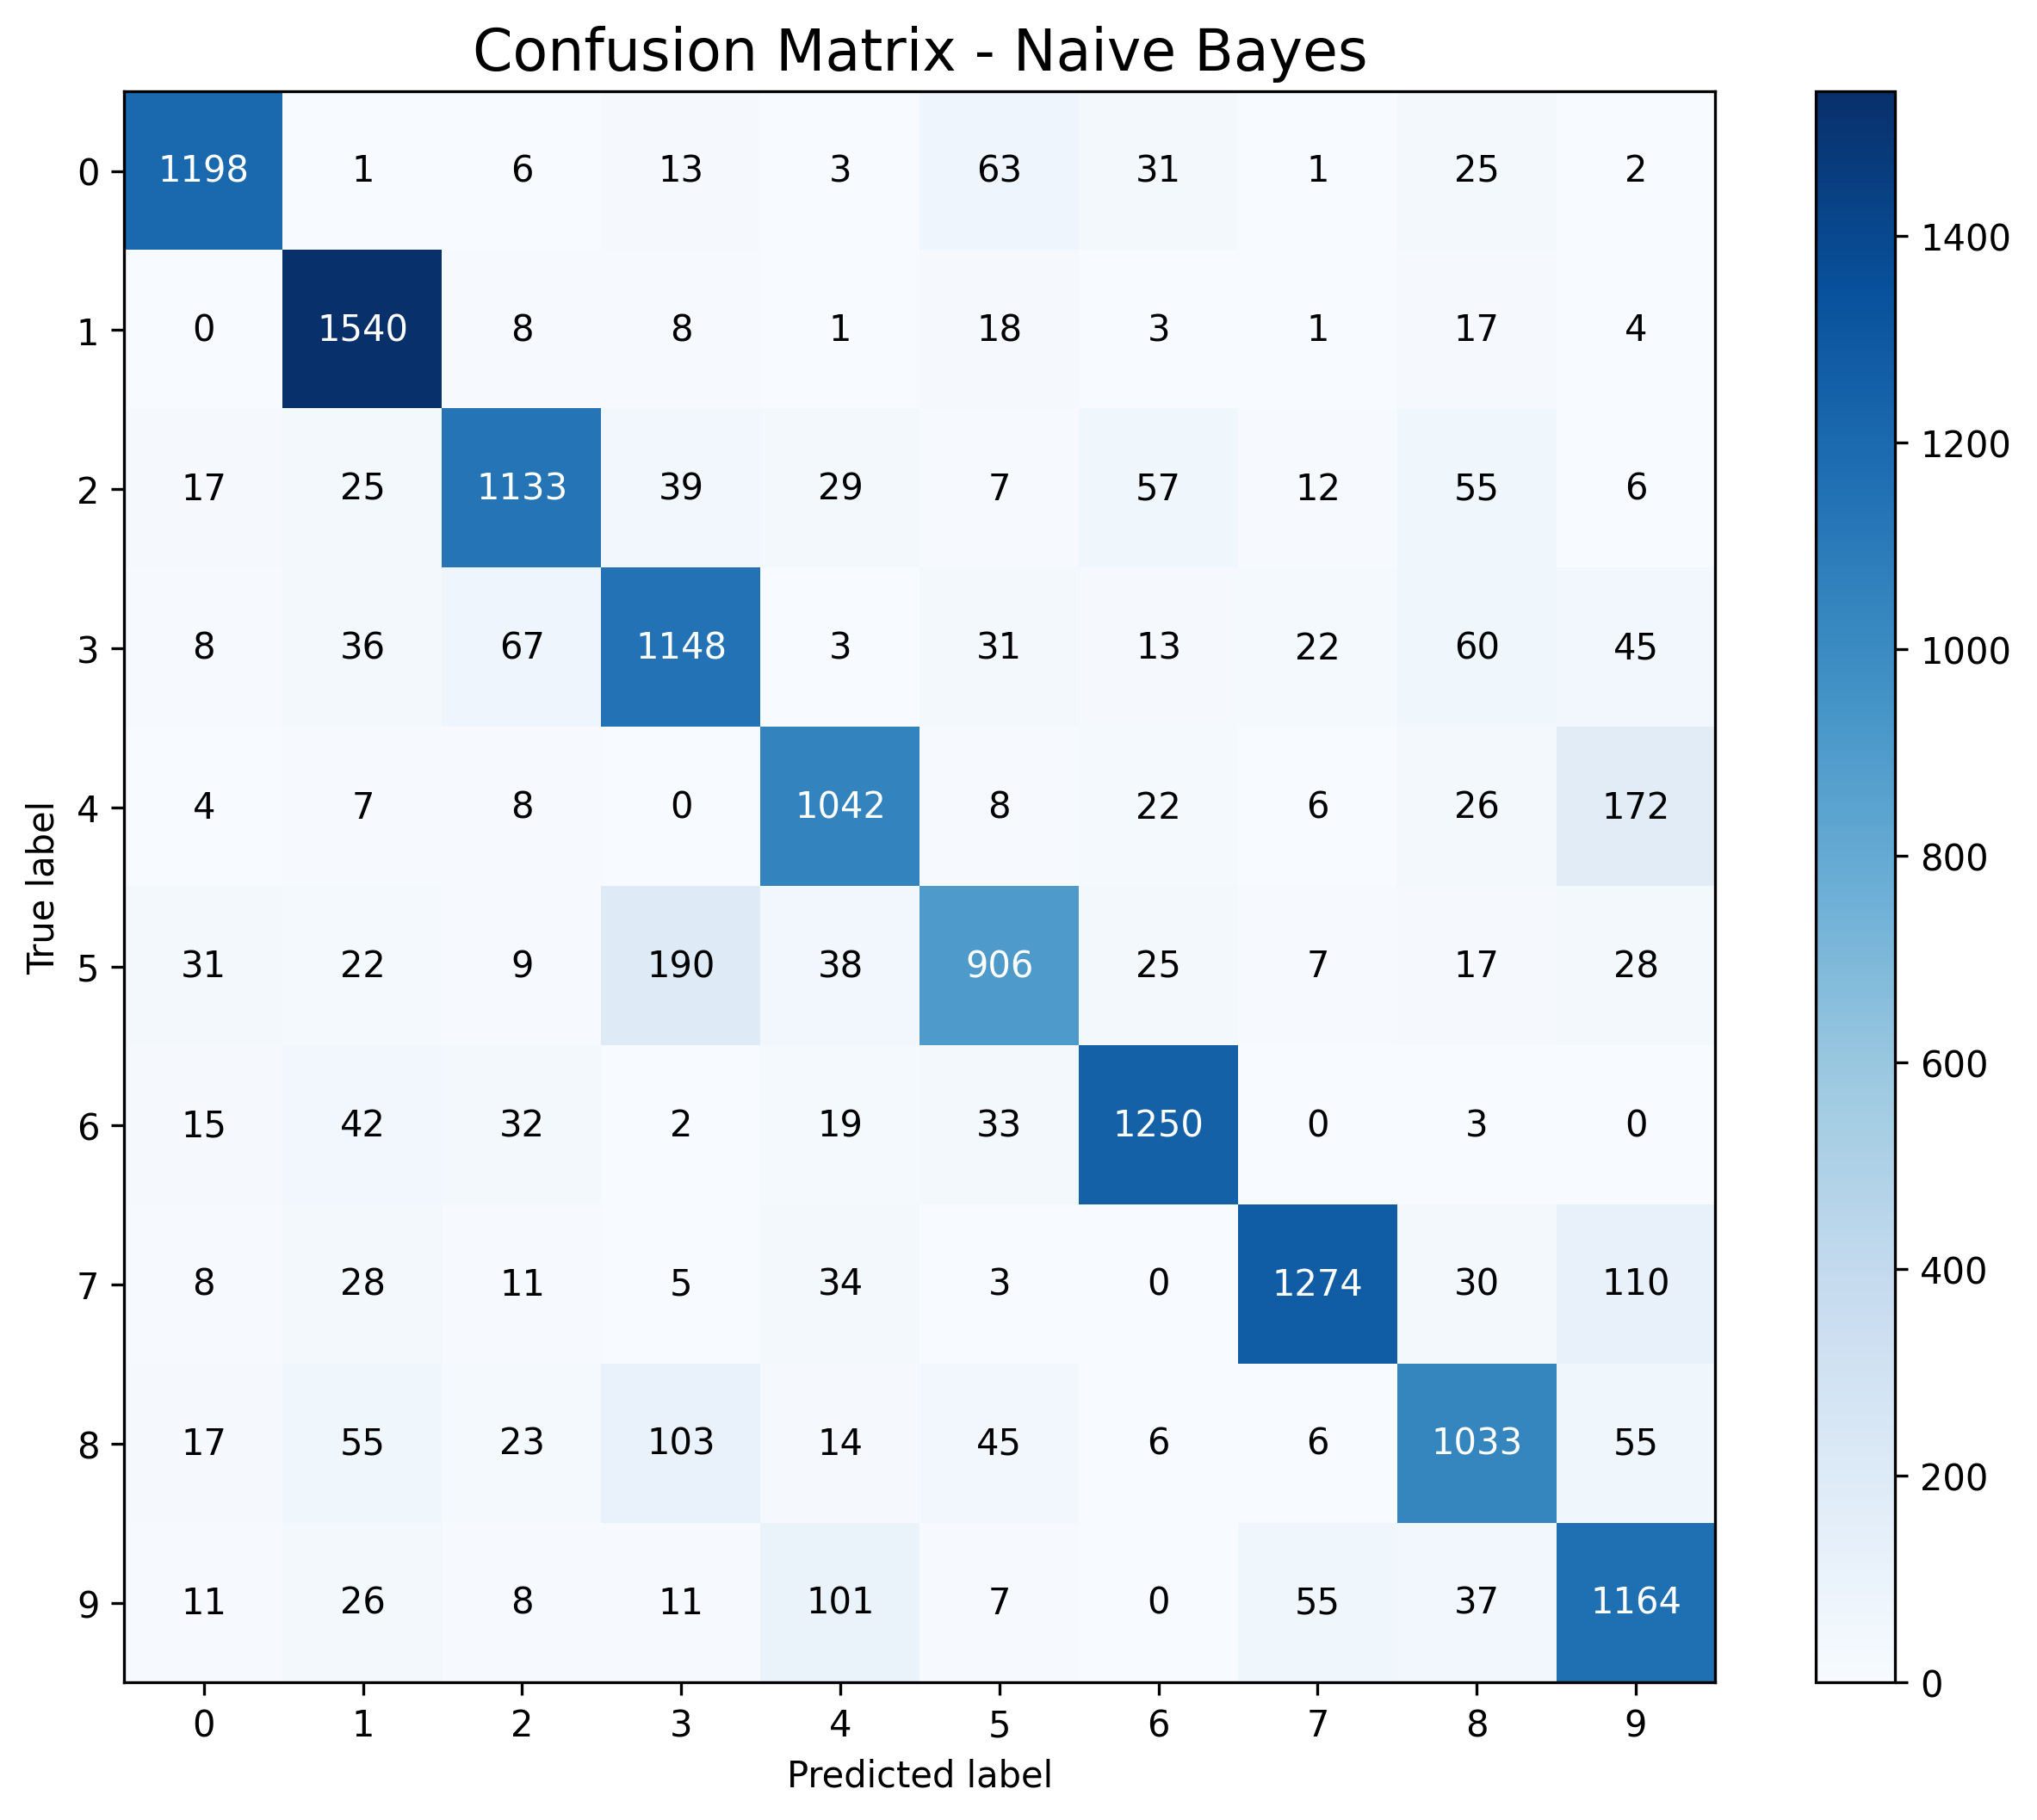
\includegraphics[width=0.8\textwidth]{../figures/3/confusion_matrix_naive_bayes.png}
    \caption{Matriz de confusão do modelo Naive Bayes}
    \label{fig:confusion_matrix}
\end{figure}

\textbf{Análise dos erros mais comuns:}

\begin{table}[H]
    \centering
    \begin{tabular}{|c|c|}
        \hline
        \textbf{Classe} & \textbf{Taxa de Erro (\%)} \\
        \hline
        0               & [ERRO\_CLASSE\_0]          \\
        1               & [ERRO\_CLASSE\_1]          \\
        2               & [ERRO\_CLASSE\_2]          \\
        3               & [ERRO\_CLASSE\_3]          \\
        4               & [ERRO\_CLASSE\_4]          \\
        5               & [ERRO\_CLASSE\_5]          \\
        6               & [ERRO\_CLASSE\_6]          \\
        7               & [ERRO\_CLASSE\_7]          \\
        8               & [ERRO\_CLASSE\_8]          \\
        9               & [ERRO\_CLASSE\_9]          \\
        \hline
    \end{tabular}
    \caption{Taxa de erro por classe no modelo Naive Bayes}
    \label{tab:error_rates}
\end{table}

A classe mais confundida foi a \textbf{[CLASSE\_MAIS\_ERRADA]}. Nota-se pela matriz de confusão que parte considerável dos erros para esta classe ocorreram pois o modelo previu [CLASSES\_CONFUNDIDAS]. Provavelmente isso acontece pela semelhança dos dígitos [DIGITOS\_SIMILARES] e pelo desbalanceamento da classe [CLASSE\_MAIS\_FREQUENTE] nos dados de treino, que foi a mais frequente.

\textbf{Contagem das classes nos dados de treino:}

\begin{table}[H]
    \centering
    \begin{tabular}{|c|c|c|c|c|c|c|c|c|c|c|}
        \hline
        \textbf{Classe}   & 0          & 1          & 2          & 3          & 4          & 5          & 6          & 7          & 8          & 9          \\
        \hline
        \textbf{Contagem} & [COUNT\_0] & [COUNT\_1] & [COUNT\_2] & [COUNT\_3] & [COUNT\_4] & [COUNT\_5] & [COUNT\_6] & [COUNT\_7] & [COUNT\_8] & [COUNT\_9] \\
        \hline
    \end{tabular}
    \caption{Distribuição das classes no conjunto de treinamento}
    \label{tab:class_distribution}
\end{table}